\documentclass[a4paper,12pt]{article}

%% Language and font encodings
\usepackage[english, russian]{babel}
\usepackage[utf8x]{inputenc}
\usepackage{blindtext}
\usepackage[T1]{fontenc}
\usepackage[T2A]{fontenc}
\usepackage[a4paper,top=1.5 cm,bottom=2cm,left=3cm,right=3cm,marginparwidth=1.75cm]{geometry}
%% Useful packages
\usepackage{amsmath, amssymb}
\usepackage{wrapfig}
\usepackage{graphicx}
\usepackage[usenames]{color}
\usepackage[T1]{fontenc}
\usepackage{tikz}
\usetikzlibrary{arrows}
\usetikzlibrary{decorations.pathreplacing}
\usepackage[T2A]{fontenc}
\usepackage{color}
\usepackage{circuitikz} 
\graphicspath{{pic/}}
\definecolor{water} {rgb} {0.667, 0.855, 1}
\usepackage{pgfplots}
\usepackage{pgfplotstable}
\usetikzlibrary{circuits}
\usetikzlibrary{circuits.ee}
\usetikzlibrary{circuits.ee.IEC}
\usetikzlibrary{circuits.logic.IEC}
\usetikzlibrary{intersections}

\title{ИЗУЧЕНИЕ ПОЛЯРИЗОВАННОГО СВЕТА}
\date{Работа 4.7.3}
\author{Ляликова Ирина, Б05-911}
\begin{document}
		\vspace{0.5 cm}
	\maketitle
	\vspace{0.5 cm}
	
	\textbf{Цель работы:} ознакомление с методами получения и анализа поляризованного света.
	
	\textbf{В работе используются:} оптическая скамья с осветителем; зеленый светофильтр; два поляроида; черное зеркало; полированная эбонитовая пластинка; стопа стеклянных пластинок; слюдяные пластинки разной толщины; пластинки в $1/4$ и $1/2$ длины волны; пластинка в одну длину волны для зеленого света (пластинка чувствительного оттенка).
	
	\section*{Теоретическое введение}
	В работе изучаются свойства поляризованного света. В линейно поляризованной световой волне пара векторов $\vec{E}$ и $\vec{H}$ не изменяет с течением времени своей ориентации. Плоскость $\vec{E}$, $\vec{S}$ называется в этом случае плоскостью колебаний. Наиболее общим типом поляризации является \textit{эллиптическая поляризация}. В эллиптически поляризованной световой волне конец вектора $\vec{E}$ (в данной точке пространства) описывает некоторый эллипс.
	
	При теоретическом рассмотрении различных типов поляризации часто бывает удобно проектировать вектор $\vec{E}$ в некоторой точке пространства на два взаимно перпендикулярных направления. В том случае, когда исходная волна была поляризованной, $E_x$ и $E_y$ когерентны между собой и могут быть записаны в виде
	\begin{equation}
	\begin{cases}
	E_x = E_{x_0}\cos(kz - \omega t),\\
	E_y = E_{y_0}\cos(kz - \omega t-\varphi),
	\end{cases}
	\end{equation}
	где амплитуды $E_{x_0}$, $E_{y_0}$, волновой вектор $k$, частота $\omega$ и сдвиг фаз $\varphi$ не зависят от времени. Формулы (1) описывают монохроматический свет. Немонохроматический свет может быть представлен суммой выражений типа (1) с различными значениями частоты $\omega$.
	
	Ориентация эллипса поляризации определяется отношением амплитуд $E_{y_0}/E_{x_0}$ и разностью фаз $\varphi$. В частности, при $\varphi = 0, \pm\pi$ эллипс вырождается в отрезок прямой (линейная поляризация). При $\varphi = \pm\pi/2$ главные оси эллипса совпадают с осями $x$, $y$. Если при этом отношение амплитуд $E_{y_0}/E_{x_0} = 1$, эллипс поляризации вырождается в окружность.	
	
	В плоскости $z = z_0$ вектор $\vec{E}$ волны (1) вращается против часовой стрелки (при наблюдении навстречу волне), если $0 < \varphi < \pi$. В этом случае говорят о левой эллиптической поляризации волны. Если же
	$\pi < \varphi < 2\pi$, вращение вектора $\vec{E}$ происходит по часовой стрелке, и волна имеет правую эллиптическую поляризацию.
	
	
	В фиксированный момент времени $t = t_0$ концы вектора $\vec{E}$ при различных $z$ лежат на винтовой линии. При этом для левой эллиптической поляризации образуется левый винт, а для правой --- правый винт.
	
	\textbf{Методы получения линейно поляризованного света.} Для получения линейно поляризованного света применяются \textit{поляризаторы}. Направление колебаний электрического вектора в волне, прошедшей через поляризатор, называется \textit{разрешенным направлением поляризатора}. Всякий поляризатор может быть использован для исследования поляризованного света, т. е. в качестве анализатора. Интенсивность $I$ линейно поляризованного света после прохождения через анализатор зависит от угла, образованного плоскостью колебаний с разрешенным направлением анализатора:
	\begin{equation}
	I = I_0 \cos^2\alpha.
	\end{equation}
	Соотношение (2) носит название закона Малюса. Опишем способы получения плоскополяризованного света, используемые в работе.
	
	\textbf{Отражение света от диэлектрической пластинки}. Отраженный от диэлектрика свет всегда частично поляризован. Степень поляризации света, отраженного от диэлектрической пластинки в воздух, зависит от показателя преломления диэлектрика $n$ и от угла падения $i$. Как следует из формул Френеля, полная поляризация отраженного света достигается при падении под углом Брюстера, который определяется соотношением
	\begin{equation}
	\text{tg}i = n.
	\end{equation}
	В этом случае плоскость колебаний электрического вектора в отраженном свете перпендикулярна плоскости падения.
	
	\textbf{Преломление света в стеклянной пластинке}. Поскольку отраженный от
	диэлектрической пластинки свет оказывается частично (или даже полностью) поляризованным, проходящий свет также частично поляризуется. Преимущественное направление колебаний электрического вектора
	в прошедшем свете совпадает с плоскостью преломления луча. Максимальная поляризация проходящего света достигается при падении под
	углом Брюстера. Для увеличения степени поляризации преломлённого
	света используют стопу стеклянных пластинок, расположенных под углом Брюстера к падающему свету.
	
	\textbf{Преломление света в двоякопреломляющих кристаллах}. Некоторые кристаллы обладают свойством двойного лучепреломления. Это связано с различием поляризуемости молекул в разных направлениях (диэлектрическая проницаемость $\varepsilon$ определяет показатель преломления среды $n$).
	Двоякопреломляющий кристалл называют одноосным, если в нём существует одно направление с экстремальным значением $\varepsilon$, а в других (перпендикулярных) направлениях значения $\varepsilon$ одинаковы. Направления вдоль осей эллипсоида называют главными, одно из них --- c экстремальным значением $\varepsilon$ --- оптической осью. Преломляясь в таких кристаллах, световой луч разделяется на два луча со взаимно перпендикулярными плоскостями колебаний. Отклоняя	один из лучей в сторону, можно получить плоскополяризованный свет, --- так устроены поляризационные призмы (Николя, Глана).
	
	\section*{Ход работы}
	В работе предлагается с помощью чёрного зеркала определить разрешённые направления поляроидов; определить характер поляризации света, прошедшего стопу и отражённого от неё под углом Брюстера; оценить угол Брюстера для эбонита; выделить пластинки $\lambda/2$ и $\lambda/4$; определить направления большей и меньшей скоростей для пластинки $\lambda/4$; исследовать интерференцию поляризованных лучей.
	\subsection*{Определение разрешённых направлений поляроидов}
	\begin{enumerate}
		\item Разместили на оптической скамье осветитель $\vec{S}$, поляроид $P_1$ и чёрное зеркало (пластинку чёрного стекла) так, чтобы плоскость падения была горизонтальна (рис. 1). Поворачивая поляроид вокруг направления луча, добились наименьшей яркости отражённого пятна. Оставили поляроид в этом положении и вращением зеркала вокруг вертикальной оси нашли положение минимальной интенсивности отражённого луча. Определили разрешённое направление поляроида (горизонтальная плоскость в данном случае).
		\begin{figure}
		\centering
		    \begin{tikzpicture}
		    \draw (0,0) rectangle (0.2,1) node[right]{$P_1$};
		    \draw (0,0) -- (0.2,1);
		    \draw (-3, 0.5) -- (3, 0.5);
		    \draw (-3, 0.5) node{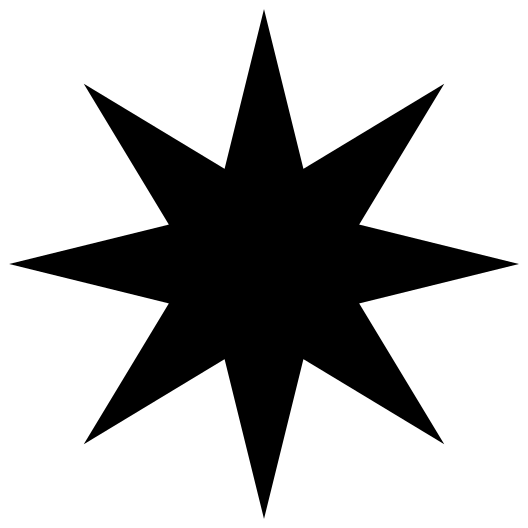
\includegraphics[width=0.5cm]{star.png}};
		    \draw (-3.3, 0.5) node[left]{$S$};
		    \draw[rotate around={65:(3.1, 0.5)}, fill] (3.1, -0.2) rectangle (3.2, 1.2) node[above right]{ЧЗ};
		    \draw[rotate around={65:(3.1, 0.5)}, dashed] (2.6, 0.5) -- (3.6, 0.5);
		    \draw[rotate around={130:(3.1, 0.5)}] (2, 0.5) -- (3.1, 0.5);
		    \begin{scope} [rotate around={130:(3.1, 0.5)}]
		        \draw (1.3, 0.5) -- (1.6, 0.8);
		        \draw (1.3, 0.5) -- (1.6, 0.2);
		        \draw (1.5, 0.3) arc (-45:45:0.28);
		    \end{scope}
		    \end{tikzpicture}
		    \caption{Схема с чёрным зеркалом}
		\end{figure}
		
		Отсчёт по лимбу поляроида $P_1$, соответствующий найденному разрешённому направлению: $\alpha_1=85^\circ$.
				
				
		Разрешённое направление второго поляроида можно определить, скрестив поляроиды как на рис. 2. Таким образом определили отсчёт по лимбу для разрешённого направления $\alpha_2=5^\circ$.
		\begin{figure}
		\centering
		    \begin{tikzpicture}
		    \draw (-0.5,0) rectangle (-0.3,1)node[right]{$P_1$};
		    \draw (0.5,0) rectangle (0.7,1) node[right]{$P_2$};
		    \draw (-0.5,0) -- (-0.3,1);
		    \draw (0.5,1) -- (0.7,0);
		    \draw (-3, 0.5) -- (3, 0.5);
		    \draw (-3, 0.5) node{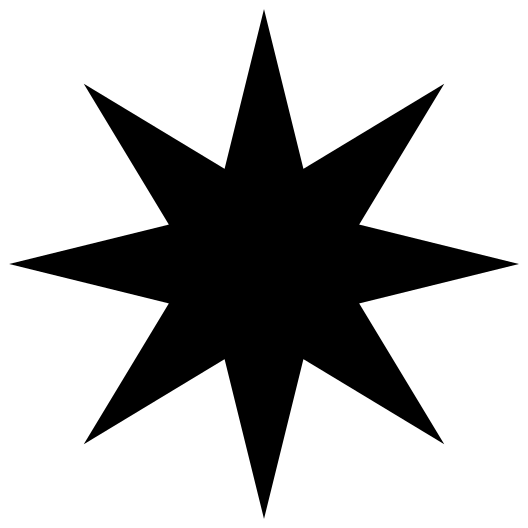
\includegraphics[width=0.5cm]{star.png}};
		    \draw (-3.3, 0.5) node[left]{$S$};
		    \begin{scope} [rotate around={180:(2.4, 0.5)}]
		        \draw (1.3, 0.5) -- (1.6, 0.8);
		        \draw (1.3, 0.5) -- (1.6, 0.2);
		        \draw (1.5, 0.3) arc (-45:45:0.28);
		    \end{scope}
		    \end{tikzpicture}
		    \caption{Схема со скрещенными поляроидами}
		\end{figure}
		
	\end{enumerate}
	\subsection*{Определение угла Брюстера для эбонита}
	\begin{enumerate}
		\item Поставили на скамью вместо чёрного зеркала (рис. 1) эбонитовую пластину с круговой шкалой.
		
		\item Повернули эбонитовое зеркало вокруг вертикальной оси так, чтобы его плоскость была перпендикулярна лучу, и совместили отражённое от эбонита пятно с отверстием осветителя (это можно сделать только в полной темноте, поэтому установили перпендикулярность на глаз). Отметили начало отсчёта по лимбу: $\alpha_3=0^\circ$.
		
		\item Установили направление разрешённых колебаний поляроида $P_1$  горизонтально и нашли угол поворота эбонита $\varphi_\text{Б}$, при котором интенсивность отражённого луча минимальна: $\varphi_\text{Б$_1$}=57^\circ$.
		
		Повторили измерения, добавив светофильтр Ф: $\varphi_\text{Б$_2$}=55^\circ$, учитывая погрешность эксперимента, значения угла с фильтром и без него отличаются незначительно.
		
		\item По углу Брюстера рассчитали показатель преломления эбонита и сравнили с табличным:
		\begin{equation*}
		    \text{tg}\varphi_\text{Б}=n_\text{эксп}\approx 1{,}5,\;\;\;\;\;\;\;n_\text{табл}\approx 1{,}6.
		\end{equation*}
	\end{enumerate}
	\subsection*{Исследование стопы}
	\begin{enumerate}
		\item Поставили стопу стеклянных пластинок вместо эбонитового зеркала и подобрали для неё такое положение, при котором свет падает на стопу под углом Брюстера. Осветили стопу неполяризованным светом и, рассматривая через поляроиды (рис. 3) свет, отражённый от стопы, определили ориентацию вектора $\vec{E}$ в отражённом луче; затем определили характер поляризации света в преломлённом луче: отражённый луч поляризован в вертикальной плоскости, преломлённый поляризован нелинейно, так как при повороте поляроида он становится тусклее, но не исчезает полностью.
		\begin{figure}
		\centering
		    \begin{tikzpicture}
		    \draw (-1.5,0) rectangle (-1.3,1) node[right]{Ф};
		    \draw (-3, 0.5) -- (3.5, 0.5);
		    \draw (-3, 0.5) node{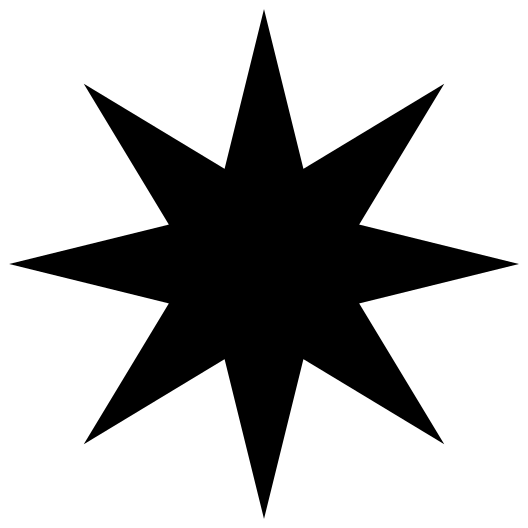
\includegraphics[width=0.5cm]{star.png}};
		    \draw (-3.3, 0.5) node[left]{$S$};
		    \begin{scope}[rotate around={65:(1, 0.5)}]
		        \draw (1, -0.2) rectangle (1.05, 1.2);
		        \draw (1.05, -0.2) rectangle (1.1, 1.2);
		        \draw (1.1, -0.2) rectangle (1.15, 1.2) node[above right]{С};
		    \end{scope}
		    \draw[rotate around={65:(1, 0.5)}, dashed] (0.5, 0.5) -- (1.5, 0.5);
		    \draw[rotate around={130:(1, 0.5)}] (-1.4, 0.5) -- (1, 0.5);
		    \begin{scope} [rotate around={130:(1, 0.5)}]
		        \draw (-2, 0.5) -- (-1.7, 0.8);
		        \draw (-2, 0.5) -- (-1.7, 0.2);
		        \draw (-1.8, 0.3) arc (-45:45:0.28);
		        \draw (-0.5, 0) rectangle (-0.3, 1) node[below left]{$P_1$};
		        \draw (-0.5, 0) -- (-0.3, 1);
		    \end{scope}
		    \begin{scope} [rotate around={180:(1, 0.5)}]
		        \draw (-2, 0.5) -- (-1.7, 0.8);
		        \draw (-2, 0.5) -- (-1.7, 0.2);
		        \draw (-1.8, 0.3) arc (-45:45:0.28);
		        \draw (-0.5, 1) rectangle (-0.3, 0) node[above right]{$P_2$};
		        \draw (-0.5, 0) -- (-0.3, 1);
		    \end{scope}
		    \end{tikzpicture}
		    \caption{Исследование стопы}
		\end{figure}
	\end{enumerate}
	\subsection*{Определение главных плоскостей двоякопреломляющих пластин}
	\begin{enumerate}
		\item Поставили кристаллическую пластинку между скрещенными поляроидами $P_1$ и $P_2$ (рис. 4). Вращая пластинку вокруг направления луча и наблюдая за интенсивностью света, проходящего сквозь второй поляроид, определили, что при углах $0^\circ, 90^\circ, 180^\circ$ и $270^\circ$ главные направления пластинки совпадают с разрешёнными направлениями поляроидов, и наблюдаемая освещённость минимальна.
		\begin{figure}
		\centering
		    \begin{tikzpicture}
		    \draw (-1.6,0) rectangle (-1.4,1)node[right]{$P_1$};
		    \draw (1.4,0) rectangle (1.6,1) node[right]{$P_2$};
		    \draw (-1.4,0) -- (-1.6,1);
		    \draw (-0.1,0) rectangle (0.1,1) node[right]{Пл};
		    \draw (1.4,0) -- (1.6,1);
		    \draw (-3, 0.5) -- (3, 0.5);
		    \draw (-3, 0.5) node{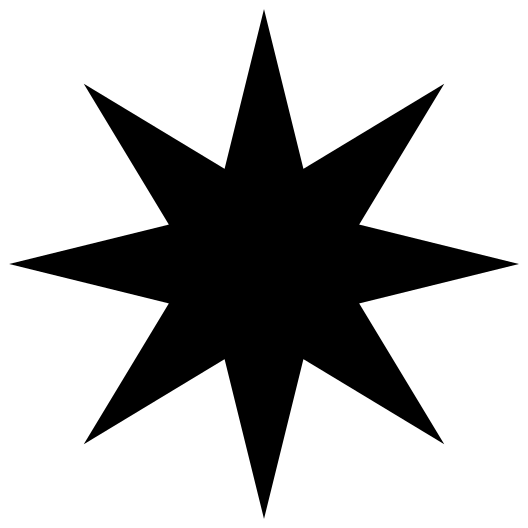
\includegraphics[width=0.5cm]{star.png}};
		    \draw (-3.3, 0.5) node[left]{$S$};
		    \begin{scope} [rotate around={180:(2.4, 0.5)}]
		        \draw (1.3, 0.5) -- (1.6, 0.8);
		        \draw (1.3, 0.5) -- (1.6, 0.2);
		        \draw (1.5, 0.3) arc (-45:45:0.28);
		    \end{scope}
		    \end{tikzpicture}
		    \caption{Определение главных плоскостей двоякопреломляющих пластин}
		\end{figure}
		
		Повторили опыт для второй пластинки.
		
	\end{enumerate}
	\subsection*{Выделение пластин $\lambda/2$ и $\lambda/4$}
	\begin{enumerate}
	    \item Добавили к схеме, изображённой на рис. 4, зелёный фильтр; установили разрешённое направление поляроида горизонтально, а главные направления исследуемой пластинки --- под углом $45^\circ$ к горизонтали.
	
	\item С помощью второго поляроида установили, какую поляризацию имеет свет, прошедший пластинку: круговую или линейную с переходом в другой квадрант. Для первой пластинки при вращении поляроида освещённость меняется, но свет не исчезает полностью, следовательно, поляризация не линейная, а круговая, и толщина пластинки $\lambda /4$. Во втором случае при поворотах поляроида освещённость падает до нуля, следовательно, поляризация линейная, и толщина второй пластинки $\lambda /2$.
	\end{enumerate}
	\subsection*{Определение направлений большей и меньшей скорости в пластинке $\lambda/4$}
	\begin{enumerate}
		\item Поставили между скрещенными поляроидами пластинку чувствительного оттенка ($\lambda$ для зелёного света), имеющую вид стрелки. Световой вектор, ориентированный вдоль направления стрелки, проходит с большей скоростью, перпендикулярный --- с меньшей.
		
		Установили разрешённое направление первого поляроида горизонтально 	и убедились с помощью второго поляроида, что эта пластинка не меняет поляризацию зелёного света в условиях предыдущего опыта.
		
		\item Убрали зелёный фильтр и поставили между скрещенными поляроидами пластинку $\lambda$ (стрелка под углом $45^\circ$ к разрешённым направлениям поляроидов). Глядя сквозь второй поляроид на стрелку, убудились, что она имеет пурпурный цвет. Это связано с тем, что зелёный свет задерживается вторым поляроидом, а красная и синяя компоненты проходят.
		
		\item Добавили к схеме пластинку $\lambda/4$ (рис. 5), главные направления которой совпадают с главными направлениями пластины $\lambda$ и ориентированы под углом $45^\circ$ к разрешённым направлениям скрещенных поляроидов. При повороте рейтера со стрелкой на $180^\circ$ вокруг вертикальной оси цвет стрелки меняется от зелёно-голубого до оранжево-жёлтого. При совпадении быстрой оси стрелки и главного направления пластинки суммарная разность хода для зеленого света составит $5\lambda/4$, что приблизительно равно длине волны в красном спектре, поэтому красный свет будет задерживаться поляроидами, что объясняет зелёно-голубой цвет стрелки. При совпадении медленой оси с главным направлением пластинки разность хода $3\lambda /4$ будет составлять длину волны для фиолетово-голубой части спектра, поэтому в результате увидим оранжево-жёлтый цвет.
		\begin{figure}
		\centering
		    \begin{tikzpicture}
		    \draw (-1.8,0) rectangle (-1.6,1)node[right]{$P_1$};
		    \draw (1.6,0) rectangle (1.8,1) node[right]{$P_2$};
		    \draw (-1.6,0) -- (-1.8,1);
		    \draw (-0.6,1) rectangle (-0.4,0) node[below ]{$\lambda$};
		    \draw (0.6,1) rectangle (0.4,0) node[below right]{$\lambda /4$};
		    \draw (1.6,0) -- (1.8,1);
		    \draw (-3, 0.5) -- (3, 0.5);
		    \draw (-3, 0.5) node{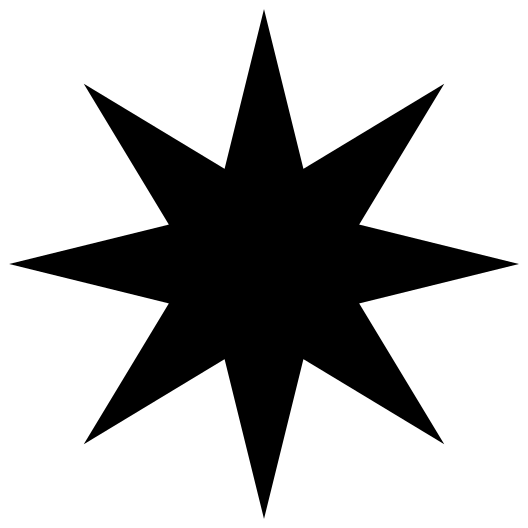
\includegraphics[width=0.5cm]{star.png}};
		    \draw (-3.3, 0.5) node[left]{$S$};
		    \begin{scope} [rotate around={180:(2.4, 0.5)}]
		        \draw (1.3, 0.5) -- (1.6, 0.8);
		        \draw (1.3, 0.5) -- (1.6, 0.2);
		        \draw (1.5, 0.3) arc (-45:45:0.28);
		    \end{scope}
		    \end{tikzpicture}
		    \caption{Определение направлений большей и меньшей скорости}
		\end{figure}
		
		\vspace{1cm}
	\end{enumerate}
	\subsection*{Определение направления вращения светового вектора в эллиптически поляризованной волне}
	\begin{enumerate}
		\item Нарисовали эллипс поляризации для вектора	$\vec{E}$, вышедшего из пластинки $\lambda/4$, где большей скорости соответствует ось $x$, а также две вышедших из пластинки синусоиды: $x(t)$ и $y(t)$ со сдвигом фаз в четверть периода (рис. 6). Проанализировали графики и определили направление вращения электрического вектора в эллиптически поляризованной волне. 
		\begin{figure}
		    \centering
		    \begin{tikzpicture}[>=latex', scale=0.7]
		        \draw[->] (-3,0) -- (3, 0)node[below]{$x$};
		        \draw[->] (0,-2) -- (0, 2)node[left]{$y$};
		        \draw (0,0) ellipse (2.2 and 1.4);
		        \draw[->] (2.2, 0) -- (2.2, 0.001);
		        \draw[->] (-2.2, 0) -- (-2.2, -0.001);
		        \draw[->] (0, 1.4) -- (-0.001, 1.4);
		        \draw[->] (0, -1.4) -- (0.001, -1.4);
		        \begin{scope}[xshift=280]
		        \clip (-4,-3) rectangle (4.5, 3);
		        \draw (0, 0) sin (-1.57,-1.3);
		        \draw (0, 0) sin (1.57,1.3);
		        \draw (3.14, 0) sin (1.57, 1.3);
		        \draw (-3.14, 0) sin (-1.57, -1.3);
		        \draw (-4.71, 1.3) cos (-3.14, 0);
		        \draw (3.14, 0) sin (4.71, -1.3);
		        \begin{scope}[xshift=0.785cm]
		        \draw (0, 0) sin (-1.57,-1.3);
		        \draw (0, 0) sin (1.57,1.3);
		        \draw (3.14, 0) sin (1.57, 1.3);
		        \draw (-3.14, 0) sin (-1.57, -1.3);
		        \draw (-4.71, 1.3) cos (-3.14, 0);
		        \draw (3.14, 0) sin (4.71, -1.3);
		        \draw (-3.5, 0.8) --++ (0.5, 0.5) node[right]{$y(t)$};
		        \draw (-3.5, -0.8) --++ (-0.5, -0.5) node[below]{$x(t)$};
		        \end{scope}
		        \draw[->] (-4,0) -- (4.5, 0)node[above left]{$t$};
		        \draw[->] (0,-2) -- (0, 2)node[left]{$E$};
		        \draw (0, -0.1) -- (0,0.1) node[anchor=south east,fill=white] {0};
		        \draw (0.785, 0.1) -- (0.785, -0.1) node[anchor=north west,fill=white] {$\frac{T}{4}$};
		        \draw (3.14, 0.1) -- (3.14, -0.1) node[anchor=north east,fill=white] {$T$};
		        \end{scope}
		    \end{tikzpicture}
		    \caption{Эллипс поляризации и две синусоиды}
		\end{figure}
		
		\item Снова поставили зелёный фильтр, а за ним между скрещенными поляроидами --- пластинку произвольной толщины.
		\item Получили эллиптически-поляризованный свет. Для этого установили разрешённое направление первого поляроида под углом 10–20$^\circ$ к горизонтали так, чтобы вектор $\vec{E}$ падающего на пластинку света был расположен в первом квадранте. Установили разрешённое направление второго поляроида вертикально и, вращая пластинку, нашли минимальную интенсивность света, прошедшего второй поляроид. Вращая второй поляроид, убедились, что свет поляризован эллиптически, а не линейно. Таким образом получили эллипс поляризации с вертикально ориентированной малой осью.
		\item Для определения направления вращения светового вектора в эллипсе 	установили между поляроидами дополнительную пластинку $\lambda/4$ с известными направлениями «быстрой» и «медленной» осей, ориентированными по осям эллипса поляризации анализируемого света. В этом случае вектор $\vec{E}$ на выходе такой, как если бы свет прошёл две пластинки $\lambda/4$: свет на выходе из второй пластинки будет линейно поляризован. Если пластинки поодиночке дают эллипсы, вращающиеся в разные стороны, то поставленные друг за другом, они скомпенсируют разность фаз, и вектор $\vec{E}$ на выходе останется в первом и третьем квадрантах. Если же световой вектор перешёл в смежные квадранты, значит, эллипсы вращаются в одну сторону. А как вращается эллипс в пластинке $\lambda/4$, определили в п. 1.
	\end{enumerate}
	\subsection*{Интерференция поляризованных лучей}
	\begin{enumerate}
		\item Расположили между скрещенными поляроидами мозаичную слюдяную 	пластинку. Она собрана из 4-х узких полосок слюды, лежащих по сторонам квадрата (две полоски «толщиной» $\lambda/4$ и по одной --- $\lambda/2$ и $3\lambda/4$). В центральном квадратике слюды нет. Главные направления всех пластинок ориентированы параллельно сторонам квадрата. Вращая пластинку, наблюдали изменения (цвета или интенсивности) в отдельном квадратике. Потом, не трогая пластинки, вращали второй поляроид. Наблюдаемые эффекты:
		\begin{itemize}
		    \item Вращаем пластинку: изменяется интенсивность света с периодичностью $\pi/4$;
		    \item Вращаем второй поляроид: изменяется (инверсируется) цвет пластинок также с периодичностью  $\pi/4$. Соответствие ячеек пластинки и разностей хода:
		    \begin{center}
		        \begin{tabular}{ |c|c|c|}
		        \hline
		        $3\lambda/4$ зелёный & $\lambda/2$ пурпурный & $3\lambda/4$ зелёный\\
		        \hline
		        $\lambda/4$ красный & - & $\lambda/4$ красный \\
		        \hline
		        $\lambda$ жёлтый & $3\lambda/4$ синий & $\lambda$ жёлтый \\
		        \hline
		        \end{tabular}
		    \end{center}
		\end{itemize}
	\end{enumerate}
	
\section*{Вывод}
Изучили явления связанные с поляризацией света: определили разрешённые направления поляроидов и с помощью них проводили следующие опыты. Рассмотрели угол Брюстера, с помощью него определили показатель преломления эбонита. Для двоякопреломляющих пластин определили главные направления, а так же тип пластинок --- $\lambda /4$ и $\lambda/2$. Также исследовали пластинку чувствительного оттенка, определили быструю и медленную оси и рассмотрели эффекты, происходящие при прохождении света через комбинацию пластинок. Получили эллиптически поляризованную волну, рассмотрели интерференцию поляризованных лучей в мозаичной слюдяной пластинке.
	
\end{document}
